\documentclass[parskip=full]{scrartcl}
\usepackage[utf8]{inputenc}
\usepackage[landscape, margin=1.5cm]{geometry}
\usepackage[scaled]{helvet} % Utilisez ce package
\renewcommand\familydefault{\sfdefault} % Définissez la police par défaut en Arial
\usepackage{multicol}
\usepackage{eso-pic}
\usepackage{tikz}
\usepackage{setspace}
\usepackage{pbox}
\usepackage{adjustbox}  
\usepackage{scrlayer-scrpage}

\usetikzlibrary{shapes.misc}

\addtokomafont{section}{\color{darkgray}}
\addtokomafont{subsection}{\color{darkgray}}

\pagenumbering{gobble}

\newcommand{\roundedtable}[1]{
    \begin{tikzpicture}
        \node[inner sep=0pt] (table) {#1};
        \draw[rounded corners=5pt] (table.north west) rectangle (table.south east);
    \end{tikzpicture}
}

\newcommand{\emptyrow}{
    \textcolor{lightgray}{\rule{0.2\textwidth}{0.1pt}} & \textcolor{lightgray}{\rule{0.14\textwidth}{0.1pt}} & \textcolor{lightgray}{\rule{0.14\textwidth}{0.1pt}} & \textcolor{lightgray}{\rule{0.14\textwidth}{0.1pt}} & \textcolor{lightgray}{\rule{0.14\textwidth}{0.1pt}} & \textcolor{lightgray}{\rule{0.14\textwidth}{0.1pt}} \\
    \hline
}

\pagestyle{scrheadings}
\chead{}
\ohead{\vspace{-15px}\hfill Nom du Manager : \textcolor{lightgray}{\rule{0.15\textwidth}{0.1pt}} - 
Date de l'Atelier : \textcolor{lightgray}{\rule{0.1\textwidth}{0.1pt}} - 
Nom de l'Équipe : \textcolor{lightgray}{\rule{0.15\textwidth}{0.1pt}}}

\AddToShipoutPictureBG{
    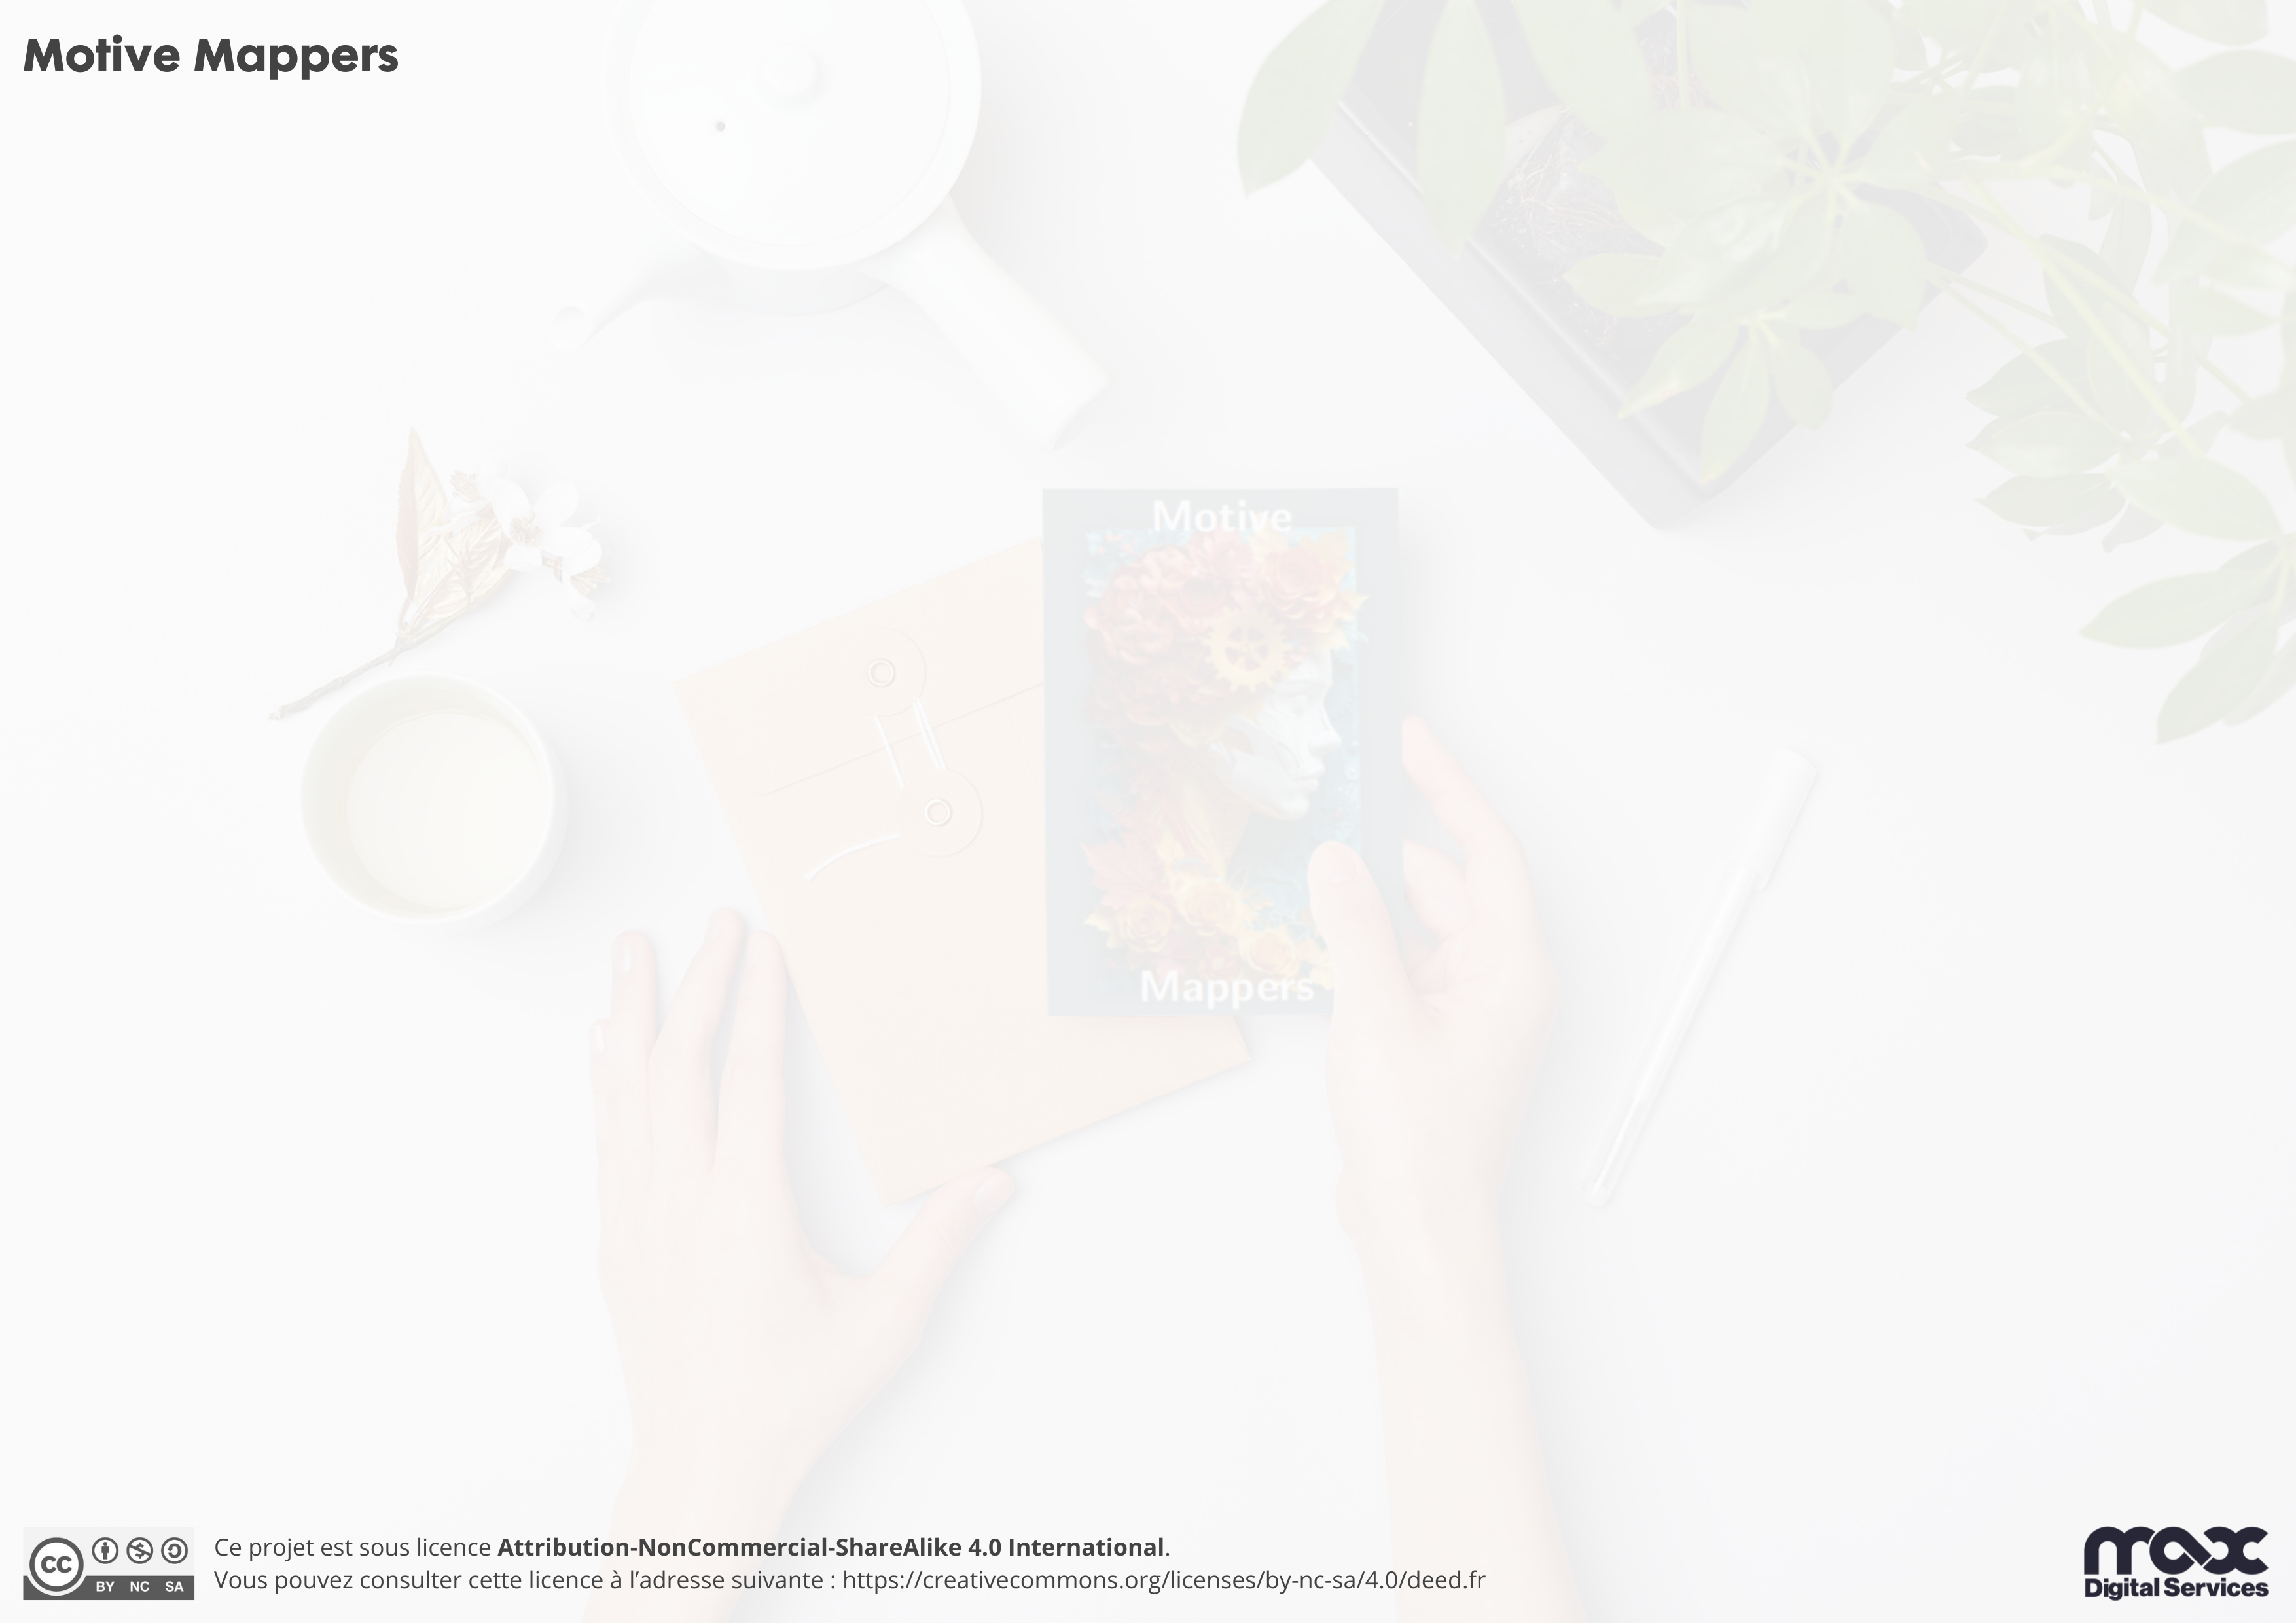
\includegraphics[width=\paperwidth,height=\paperheight]{images/background-scoring.png}
}

\thispagestyle{empty}

\title{Récapitulatif des Motivations d'Équipe}
\date{}

\begin{document}
\section*{Mode d'emploi}
\begin{minipage}[t]{\textwidth}
    \begin{multicols}{2}
        \subsection*{Instructions}
        Utilisez la \textbf{Feuille de score} pour noter les choix de chaque participant durant l'atelier \textbf{Motive Mappers}.\\

        Utiliser le tableau \textbf{Analyse des Motivations d'Équipe} pour identifier les tendances, les points forts, et les domaines à améliorer dans l'équipe.

        \subsection*{Déroulement d'une Session}

        \begin{enumerate}
            \item Expliquez brièvement chaque carte et son symbolisme.
            \item Les participants choisissent et classent leurs 5 principales motivations intrinsèques.
            \item Les participants partagent et discutent leurs choix avec le groupe.
            \item Demandez aux participants d'évaluer si les motivations sélectionnées sont présentes dans leur cadre de travail actuel, en glissant les cartes vers le haut ou le bas.
            \item Les participants identifient les tendances communes et les différences dans les motivations de l'équipe.
            \item Récapitulatif des points clés et des tendances observées.
            \item Session de questions/réponses pour clarifier ou approfondir certains aspects.
        \end{enumerate}

        \subsection*{Pour rappel}
        Voici un résumé des cartes pour "Motive Mappers" avec leurs descriptions :

        \begin{itemize}
            \item \textbf{Acceptation} : Besoin de reconnaissance et d'appréciation par les autres.
            \item \textbf{Curiosité} : Désir d'explorer et d'apprendre.
            \item \textbf{Liberté} : Aspiration à l'indépendance et au choix personnel.
            \item \textbf{Honneur} : Engagement envers les valeurs personnelles et l'éthique.
            \item \textbf{Statut} : Quête de reconnaissance sociale ou professionnelle.
            \item \textbf{Maîtrise} : Volonté d'exceller et de développer ses compétences.
            \item \textbf{But} : Désir de poursuivre un travail significatif.
            \item \textbf{Ordre} : Besoin de structure et de clarté.
            \item \textbf{Pouvoir} : Aspiration à influencer et à diriger.
            \item \textbf{Socialisation} : Importance des relations et interactions humaines.
            \item \textbf{Récompense} : Satisfaction de recevoir une compensation juste pour les efforts.
            \item \textbf{Stabilité} : Recherche de sécurité dans la vie professionnelle.
            \item \textbf{Harmonie} : Équilibre entre vie professionnelle et personnelle.
            \item \textbf{Appartenance} : Alignement avec les valeurs et la culture de l'entreprise.
            \item \textbf{Autonomie} : Désir de liberté dans l'organisation du travail.
            \item \textbf{Impact} : Volonté de contribuer positivement à la société.
            \item \textbf{Innovation} : Enthousiasme pour la nouveauté et la technologie.
            \item \textbf{Développement} : Aspiration à la croissance personnelle et professionnelle.
        \end{itemize}
        Ces cartes représentent un éventail de motivations intrinsèques, facilitant la compréhension et la discussion sur ce qui motive individuellement et collectivement dans un cadre professionnel.

    \end{multicols}
\end{minipage}

\section*{Etape 1 : Feuille de Score}
\begin{table}[h!]
    \renewcommand{\arraystretch}{1.5}
    \centering
    \begin{adjustbox}{width=0.9\textwidth,center}
        \roundedtable{
            \begin{tabular*}{\textwidth}{p{0.2\textwidth}|p{0.14\textwidth}|p{0.14\textwidth}|p{0.14\textwidth}|p{0.14\textwidth}|p{0.14\textwidth}}
                \textbf{Nom du Participant} &  5eme position & 4eme position & 3eme position & 2nd position & 1er position \\
                \hline
                \emptyrow
                \emptyrow
                \emptyrow
                \emptyrow
                \emptyrow
                \emptyrow
                \emptyrow
                \emptyrow
                \emptyrow
                \emptyrow
                \emptyrow
                \emptyrow
                \emptyrow
                \emptyrow
                \emptyrow
                \emptyrow
                \emptyrow
                \emptyrow
                \emptyrow
                \emptyrow
                \emptyrow
                \emptyrow
                \emptyrow
            \end{tabular*}
        }
    \end{adjustbox}
\end{table}

\newpage
\section*{Etape 2 : Analyse des Motivations d'Équipe}
\begin{multicols}{2}
    \begin{minipage}[t]{0.45\textwidth}
        \subsection*{Tableau de Calcul des Motivations d'Équipe}
        \renewcommand{\arraystretch}{1.5}
        \roundedtable{
            \begin{tabular*}{\textwidth}{l|c|c|c}
                \textbf{Motivation} & Nb de Mentions & Présentes (+) & Absentes (-) \\
                \hline             Acceptation         &                             &                        &                       \\
                \hline Curiosité           &                             &                        &                       \\
                \hline Liberté             &                             &                        &                       \\
                \hline Honneur             &                             &                        &                       \\
                \hline Statut              &                             &                        &                       \\
                \hline Maîtrise            &                             &                        &                       \\
                \hline But                 &                             &                        &                       \\
                \hline Ordre               &                             &                        &                       \\
                \hline Pouvoir             &                             &                        &                       \\
                \hline Socialisation       &                             &                        &                       \\
                \hline Récompense          &                             &                        &                       \\
                \hline Stabilité           &                             &                        &                       \\
                \hline Harmonie            &                             &                        &                       \\
                \hline Appartenance        &                             &                        &                       \\
                \hline Autonomie           &                             &                        &                       \\
                \hline Impact              &                             &                        &                       \\
                \hline Innovation          &                             &                        &                       \\
                \hline Développement       &                             &                        &
            \end{tabular*}
        }
    \end{minipage}

    \begin{minipage}[t]{0.45\textwidth}
        \subsection*{Observations}
        Notez ici les tendances générales, les motivations dominantes, les disparités, et tout autre observation pertinente.

        \subsubsection*{Synthèse}
        \textbf{Motivations Dominantes de l'Équipe:} \\
        \textcolor{lightgray}{\rule{\textwidth}{0.1pt}} \\
        \textcolor{lightgray}{\rule{\textwidth}{0.1pt}} \\
        \textcolor{lightgray}{\rule{\textwidth}{0.1pt}}

        \textbf{Motivations à Développer:} \\
        \textcolor{lightgray}{\rule{\textwidth}{0.1pt}} \\
        \textcolor{lightgray}{\rule{\textwidth}{0.1pt}} \\
        \textcolor{lightgray}{\rule{\textwidth}{0.1pt}}

        \subsubsection*{Actions}
        \textbf{Stratégies Proposées:} \\
        \textcolor{lightgray}{\rule{\textwidth}{0.1pt}} \\
        \textcolor{lightgray}{\rule{\textwidth}{0.1pt}} \\
        \textcolor{lightgray}{\rule{\textwidth}{0.1pt}} \\
        \textcolor{lightgray}{\rule{\textwidth}{0.1pt}} \\
        \textcolor{lightgray}{\rule{\textwidth}{0.1pt}} \\
        \textcolor{lightgray}{\rule{\textwidth}{0.1pt}}

        \subsection*{Notes Additionnelles}
        Utilisez cet espace pour toute note supplémentaire ou observation durant l'atelier.\\
        \\
        \textbf{Note :} \textcolor{lightgray}{\rule{0.9\textwidth}{0.1pt}} \\
        \textcolor{lightgray}{\rule{\textwidth}{0.1pt}} \\
        \textcolor{lightgray}{\rule{\textwidth}{0.1pt}} \\
        \textcolor{lightgray}{\rule{\textwidth}{0.1pt}}
    \end{minipage}
\end{multicols}
\end{document}